\documentclass[a4,center,fleqn]{NAR}

% Enter dates of publication
\copyrightyear{2008}
\pubdate{31 July 2009}
\pubyear{2009}
\jvolume{37}
\jissue{12}

%\articlesubtype{This is the article type (optional)}
\providecommand{\e}[1]{\ensuremath{\times 10^{#1}}}

\begin{document}

\title{\textit{dpcR}: web server and R package for analysis of digital PCR 
experiments}

\author{%
Micha\l{} Burdukiewicz\,$^{1,6}$,
Jim Huggett\,$^{2}$,
Alexandra Whale\,$^{2}$,
Bart K.M. Jacobs\,$^{3}$,
Lieven Clement\,$^{3}$,
Piotr Sobczyk\,$^{1}$,
Andrej-Nikolai Spiess\,$^{4}$,
Peter Schierack\,$^{5}$,
Stefan R\"odiger\,$^{5}$\footnote{To whom correspondence should be addressed.
Tel: +49 357385 936; Fax: +49 357385801; Email: stefan.roediger@b-tu.de}}

\address{%
$^{1}$Department of Genomics, Faculty of Biotechnology, University of 
Wroc\l{}aw, Wroc\l{}aw, Poland
and
$^{2}$Molecular and Cell Biology Team, LGC, Teddington, United Kingdom
and
$^{3}$Department of Applied Mathematics, Computer Science and Statistics, Ghent 
University, Belgium
and
$^{4}$University Medical Center Hamburg-Eppendorf, Hamburg, Germany
and
$^{5}$Institute of Biotechnology, Brandenburg University of Technology 
Cottbus~--~Senftenberg, Gro\ss{}enhainer Str. 57, 01968, Senftenberg, Germany
}
% Affiliation must include:
% Department name, institution name, full road and district address,
% state, Zip or postal code, country

\history{%
Received January 1, 2009;
Revised February 1, 2009;
Accepted March 1, 2009}

\maketitle

\begin{abstract}

The digital Polymerase Chain Reaction (dPCR) enables an absolute 
quantification of nucleic acids. Different statistical analysis frameworks
were proposed. However, most analysis is done in closed source software as 
provided by the vendors. This makes it harder to compare results, such as the 
confidence interval estimates. An unified open software framework for 
reproducible research is not available.

To perform dPCR analysis we implemented peer-review statistical methods and 
plots into the \textit{dpcR} framework, based on the sophisticated statistical 
computing environment \textbf{R}. \textit{dpcR} is versatile open source 
cross-platform software framework, which provides functions to process dPCR 
data 
independent of the hardware. Our software can be used for data analysis and 
presentation, as framework for novel technical developments and as reference 
for 
statistical methods in dPCR analysis. Features such as functions to estimate 
the 
underlying Poisson process, calculation of confidence intervals based on single 
samples as well as on replicates, a novel Generalized Linear Model-based 
procedure to compare dPCR experiments and a spatial randomness test for 
assessing plate effects have been integrated. We use a plug-in like 
architecture 
and abstraction layers to make the framework usable for droplets and 
(real-time) 
chamber based technologies.

\textit{dpcR} is implemented with interfaces to the command-line, graphical 
user interfaces and interactive web application. Therefore, it can be used by 
novices in a graphical user interface or by experts via a command-line 
interface. The \textit{dpcR} framework can be used to build a custom-made 
analyser according to the user requirements. \textit{dpcR} is an 
open framework, which can be easily adapted to the growing knowledge in dPCR. 
  
\end{abstract}


\section{Introduction}

The digital PCR (dPCR) is an important contender for precise nucleic acids 
quantifications. Application of the dPCR include investigation of allele 
frequencies, single-cell analysis, gene expression analysis and absolute 
quantification of PCR products. The chemical basis (e.g., buffer, primer) of the 
dPCR and thermal cycling is similar to the real-time quantitative qPCR (qPCR). 
Though, approaches based on isothermal amplification were also developed 
\cite{pabinger_survey_2014, ludlow_2014, rodiger_r_2015}. A first proposal for a 
dPCR-like approach and the use of the Poisson distribution to quantify the 
number of molecules on a ``sample'' was shown by Ruano \textit{et al.} 1990 
(PNAS) with the single molecule dilution (SMD) PCR \cite{ruano_haplotype_1990}. 
In 1999 Vogelstein \textit{et al.} (PNAS) described the first true dPCR 
\cite{vogelstein_digital_1999}. Since approximately ten years the dPCR is 
rapidly gaining momentum in the mainstream user-base and will likely have the 
same impact as the qPCR methodology. There is an intensive research on dPCR 
platforms with the overall aim to make to technology broadly usable, cheap, 
robust and to enable high sample throughput \cite{selck_increased_2013, 
huggett_qpcr_2015, morley_digital_2014}. 

% **************************************************************
% Keep this command to avoid text of first page running into the
% first page footnotes
\enlargethispage{-65.1pt}
% **************************************************************

On the opposite to qPCR, dPCR consists of multiple amplifications occurring in 
numerous small ``partitions'' (e.g., nL volume droplets of water oil 
emulsions, chambers on micro structured chips). The result of dPCR is a binary 
vector describing states of partitions (positive in case of detected 
amplification, negative otherwise). The amplification in positive partitions 
indicates the presence of one or more template molecules. It is assumed that 
distribution of template molecules over partitions is described appropriately 
by the Poisson distribution. This probability distribution is parametrized 
using only single parameter, $\lambda$, which may be interpreted as the mean 
number of template molecules per partition. The relationship between 
$\lambda$, the number of positive partitions $k$ and the total number of 
partitions $n$ is as follows:
\begin{equation}
 \lambda = -\log{\left( 1 - \frac{k}{n} \right)}
\end{equation}

Knowing the $\lambda$ and volume of the single partition, the computation of 
the concentration of a template in the sample seems to be trivial, yet methods 
of analysis of dPCR results are still emerging.

The variety of existing procedures is disproportionate to the number of 
software packages dedicated to analysis of dPCR experiments. Most of the 
software comes in form of closed-source packages distributed by vendors of dPCR 
systems. The proprietary software without open source code prohibits validation 
the implementation of the assumed methodology and therefore has a limited usage 
in research. Moreover, vendors usually tie tightly software with their 
hardware, which hinders a comparison of results from different systems.

The lack of a dedicated software for analysis of dPCR results leads to the rapid 
development of custom scripts in \textbf{Mathematica} (Wolfram Research) 
\cite{strain_highly_2013}, \textbf{MS EXCEL} (Microsoft) 
\cite{dobnik_multiplex_2015} or \textbf{R} \cite{trypsteen_ddpcrquant_2015, 
dreo_optimising_2014}. In addition, web-servers for analysis of dPCR data, as 
the \textbf{definetherain} \cite{jones_low_2014}, are emerging. However, these 
efforts have limited use, since they are tied to a very specific problem. Even 
if they introduce some level of abstraction, it is not documented well enough to 
permit usage in other workflows.

The described situation is unfavorable for studies involving dPCR data. The 
absence of graphical user interfaces prohibits majority of researchers from 
using the custom-made frameworks. Others have to implement methods on their own, 
shifting their focus from an investigation to programming. 

In 2013 we started the development of the \textit{dpcR} framework to perform 
analysis of dPCR experiments \cite{burdukiewicz_dpcr:_2013}. We have chosen R 
software environment \cite{Rcitation}, because it is already extensively used 
in studies of qPCR data \cite{pabinger_survey_2014, rodiger_r_2015}, both 
pre-processing (\cite{roediger2015chippcr, perkins_readqpcr_2012}) and 
analysis (\cite{rodiger_surface_2013, ritz_qpcr_2008}). Furthermore, R is 
freely available for the MacOS, Linux/Unix and Windows operating systems. It 
supports literate programming (e.g., \textit{knitr}) and tools for reproducible 
research (e.g., \textit{rctrack}) \cite{liu_r_2014}. 

Since the R's command-line interface might not meet the needs of all potential 
users, we added also a web server \textit{dpcReport} using the \textit{shiny} 
package. It allows access to the most of \textit{dpcR} functionalities through 
the Graphical User Interface (GUI). \textit{dpcReport} can be also installed as 
the stand-alone software.

\section{MATERIALS AND METHODS}

\subsection{Implementation of \textit{dpcR}}

%\textit{MBmca} \cite{rodiger_surface_2013} 
The \textit{dpcR} package is an open source extension to \textbf{R}. It 
employs object-oriented programming paradigm and the \texttt{underscore\_sep} 
naming convention \cite{Baaaath_2012}.

Any processing of dpcR data is inevitably tied to the information loss, so we 
suggest to start analysis with raw data rather than summaries exported by 
vendor-provided software. If it is not possible, part of \textit{dcpR} 
functionalities will be not available, but most of the study can be still 
successfully conducted using the same commands as in the case of unprocessed 
data. 

Such universality results from the usage of uniform data format in all 
computations inside the workflow. Datasets, regardless of their origin (array- 
or droplet-based dPCRs) and type (total number of positive partitions, states of 
partitions, CQs of partitions), are stored in the standardized class. Subclasses 
further define the more specific features of objects as the spatial organization 
of chambers in case of the array-based dPCR.

\begin{figure*}[t]
\begin{center}
%\includegraphics[page = 1, trim = 0cm 10cm 0cm 0cm, clip, 
%width=17cm]{dpcR_analysis.pdf}
\end{center}
\caption{\textit{dpcR} workflow. The diagram shows main functions 
available at each step of a dPCR data analysis.}
\label{workflow}
\end{figure*}

The workflow of \textit{dpcR} encloses complete data analysis, starting from 
data import or simulation and ending with report generation (Figure 
\ref{workflow}). The package employs peer-reviewed methods of computing the 
$\lambda$ value and assess its uncertainty. We also implemented previously 
published methods of statistical analysis of dPCR reactions.

\subsection{Data import}

Import functions limit availability of the package by determining which datasets 
can be easily processed using the provided framework. To address the needs of 
potential users, \textit{dpcR} not only covers data import from most popular 
systems, but also facilities data simulation and conversion of qPCR datasets.

Since the RDML format for dPCR is not yet established, we wrote function 
\textit{read\_dpcr} streamlining data import from several systems (see Table 
\ref{table_formats}). To cover experimental or not yet included systems, we 
created a ''raw data'' format (see Supplementary Files for description). The 
user can manually arrange his data in this format and import it to the 
\textit{dpcR} package. Such input files can be created in a spreadsheet program 
or a text editor.

\begin{table}[b]
\tableparts{%
\caption{Structured vendor export data formats handled by \textit{dpcR}~v.~0.5 
and later.} 
\label{table_formats}%
}{%
\begin{tabular*}{\columnwidth}{@{}llll@{}}
\toprule
Vendor & System & Format & Type
\\
\colrule
Bio-Rad & QX100 \& QX200 & CSV & Summary export
\\
Fluidigm & BioMark & CSV & Summary export
\\
Formulatrix & Constellation Digital PCR & CSV & Summary export
\\
\botrule
\end{tabular*}%
} {The number of structured export data formats handled by \textit{dpcR} is 
growing. CSV, comma separated values.}
\end{table}

Moreover, \textit{dpcR} accepts other \textbf{R} objects, which is useful if the 
data required some further pre-processing not covered by the package (e.g., 
removal of missing values, smoothing \cite{spiess_impact_2015}). Such objects 
may be integrated into the workflow using the \textit{df2dpcr} or more flexible 
\textit{create\_dpcr} functions.

\subsubsection{Data simulation}

We found two methods of simulating results of dPCR \cite{dube_mathematical_2008, 
jacobs_2014}. The former is based on randomly distributing the exact number 
of template molecules over defined number of identical partitions. It results in 
the vector of partitions with known number of template molecules. 

The procedure in Jacobs~\textit{et al.}~2014 models more complicated situation, 
fluorescence values of the passing droplets. The number of template molecules in 
particular partition as well as the volume of the partition are determined by 
separate probability distributions. The number of molecules per partition is 
further converted to the fluorescence values considering the random effects 
affecting amplification efficiency. The simulation also includes such phenomena 
as ``rain'', droplets that cannot be unambiguously assessed as positive or 
negative.

We complement these methods with our own, where the number of template molecules 
distributed over identical partitions is not exactly specified, but determined 
by the Poisson distribution with specific parameters. It is best described as 
the variant of procedure introduced elsewhere \cite{dube_mathematical_2008}, but 
without the assumption of having the constant number of template molecules over 
all samples. All three methods are available under \textit{sim\_dpcr} 
command.

\subsubsection{Integration of qPCR data}

High-Throughput qPCR is a well established and robust technology, which allows 
precise quantification of DNA material in high throughput fashion. However, the 
quantification by qPCR is challenging at very low and very high concentrations. 
In addition, pre-processing and data analysis is a affected by numerous adverse 
effects \cite{ruijter_2013, spiess_impact_2015}. 

The recently proposed solution \cite{mojtahedi_2014} overcomes these 
complications by using the dPCR methodology to analyze qPCR data. Briefly, 
quantification points (Cq) are computed using the real-time measurements of 
several amplification curves. Next, the Cq values are binarized and treated as 
the status of partitions effectively converting multiple qPCR experiments into a 
dPCR. This functionality is supported by the \textit{qpcr2pp} function (Figure 
\ref{qpcr2pp_1}).

\begin{figure}[t]
\begin{center}
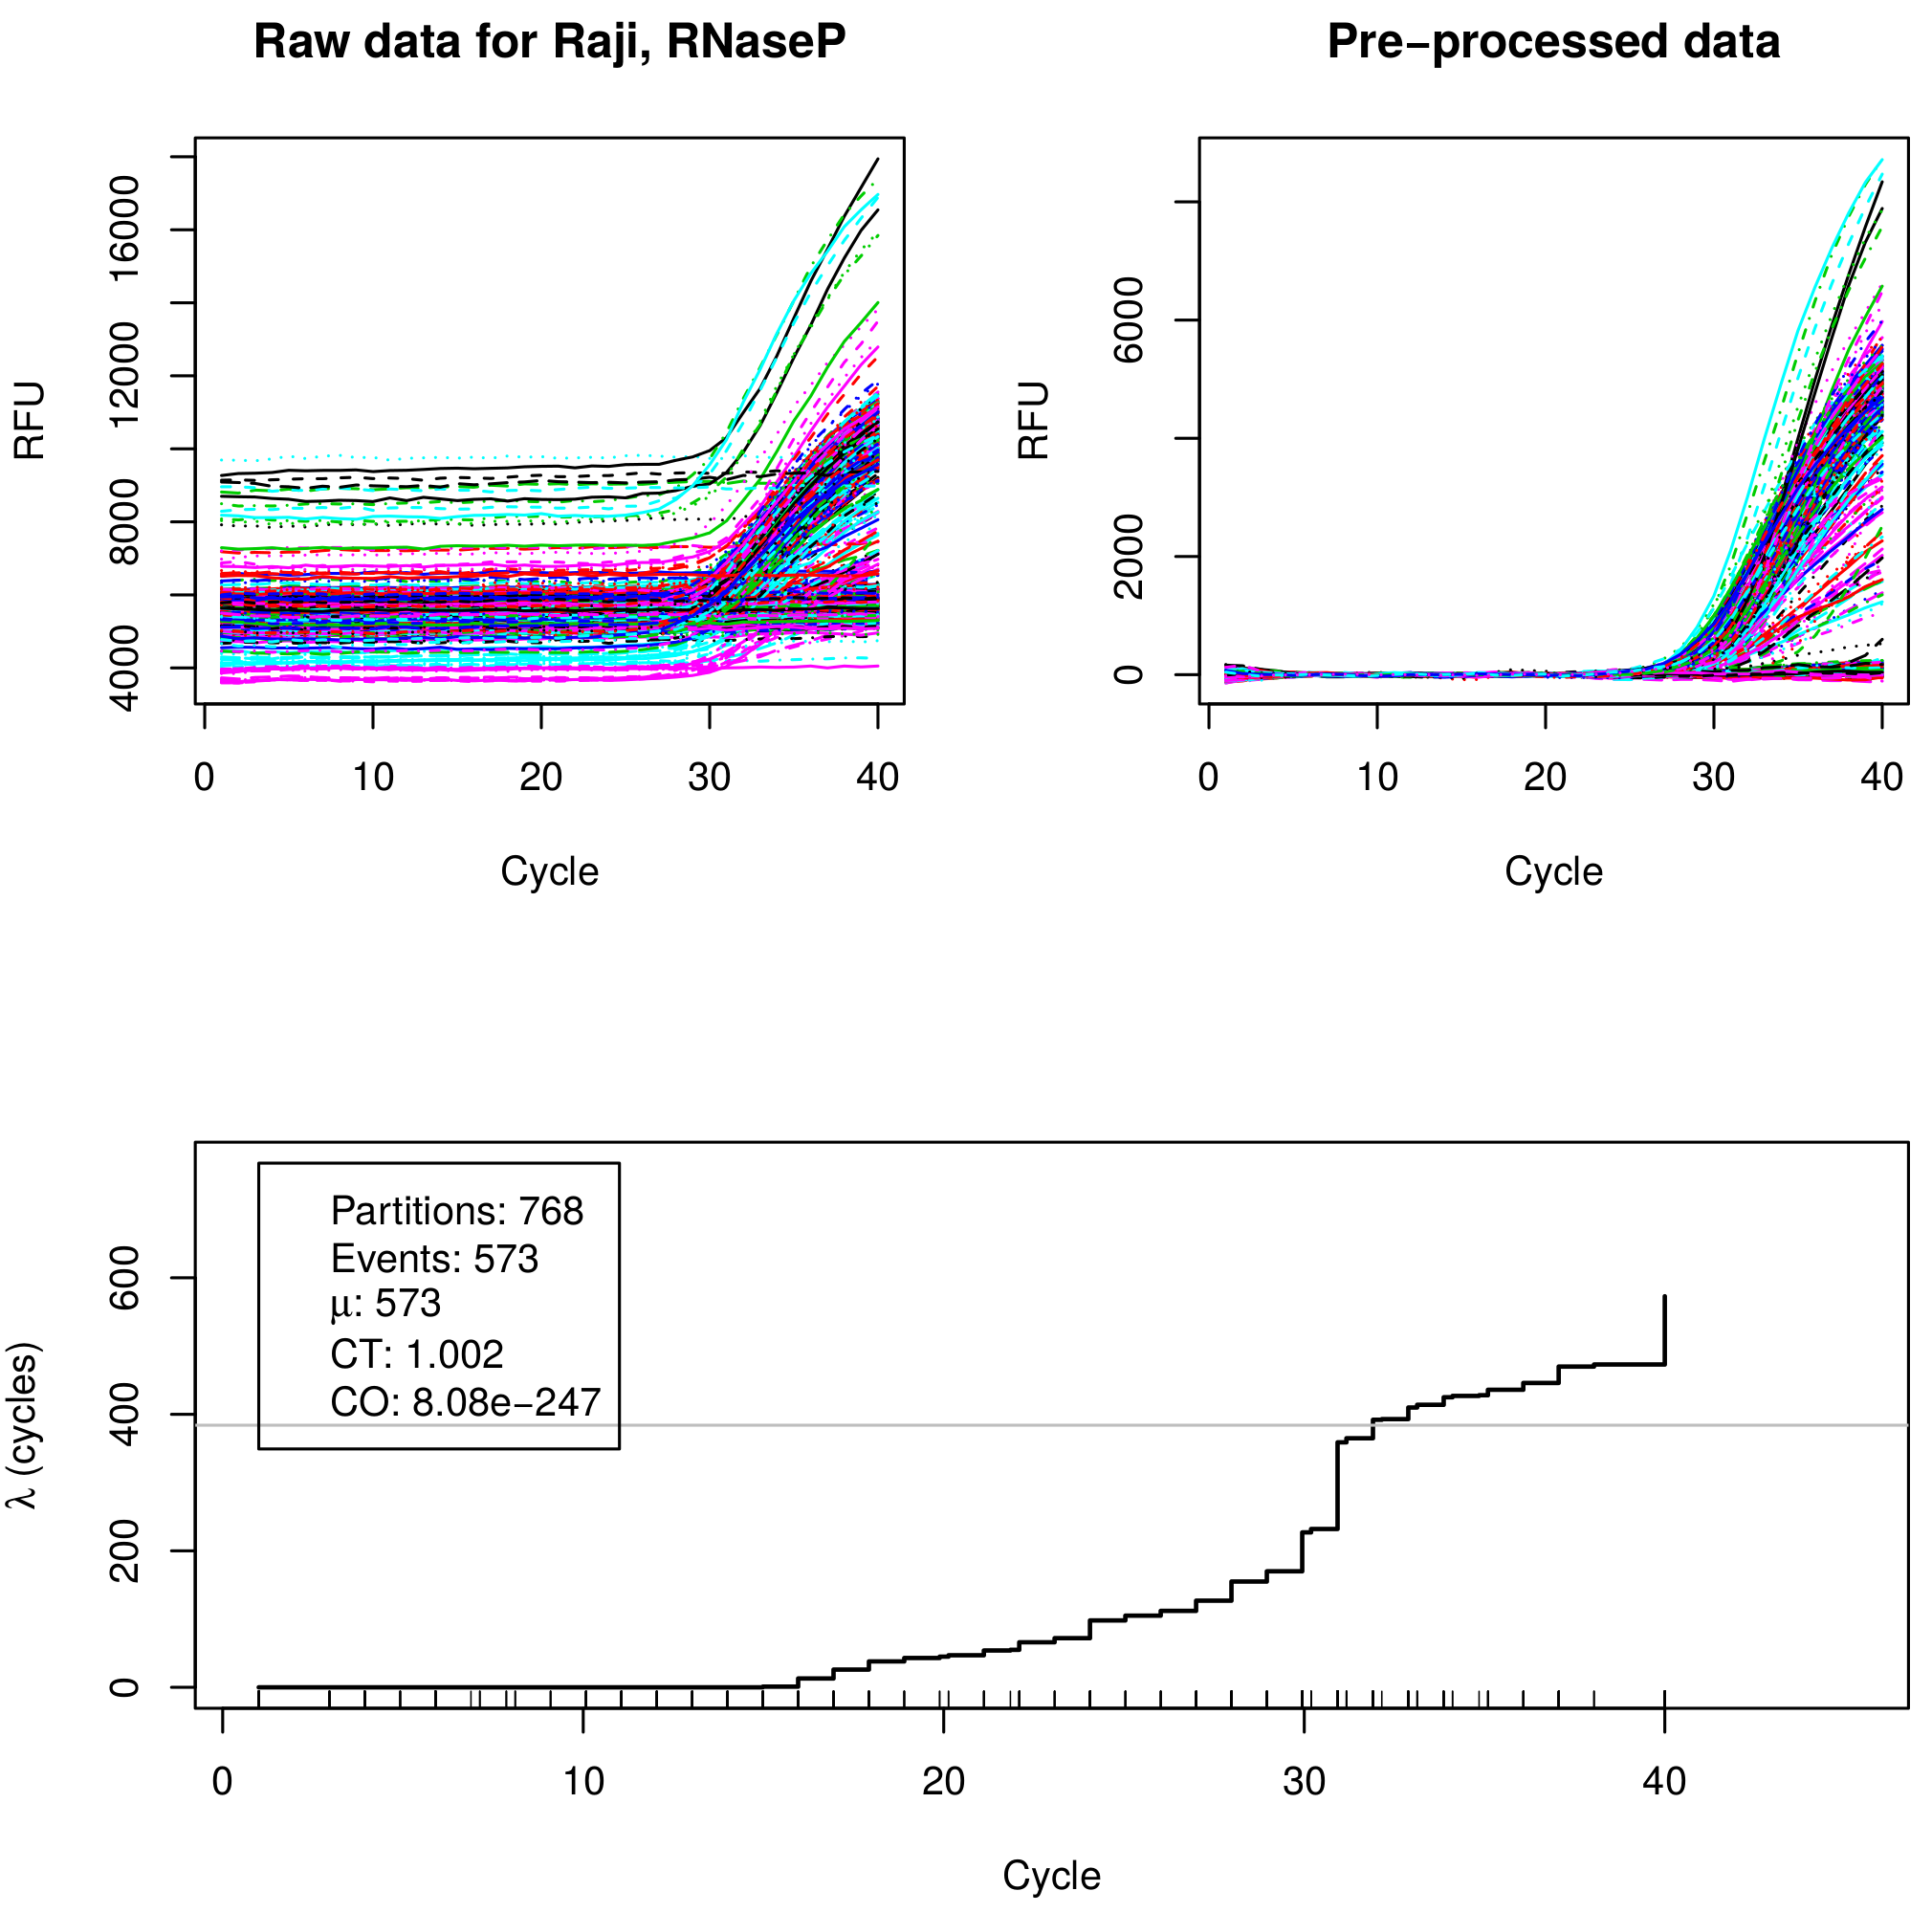
\includegraphics[width=9cm]{qpcr2pp_1.png}
\end{center}
\caption{Uncover characteristics of dPCR data. Selected dPCR platforms are qPCR 
platforms at the same time. The function \textit{qpcr2pp} uses the qPCR 
amplification curve data and interprets them as dPCR (Poisson process). A) Raw 
data of The function were B) preprocessed (baselined, smoothed) with functions 
from the \textit{chipPCR} package and C) finally analysed (Cq calculation 
$\rightarrow$ binarize) with the \textit{qpcr2pp} (qPCR to Poisson process) 
function from the \textit{dpcR} package.} 
\label{qpcr2pp_1}
\end{figure}

\subsection{Statistical analysis}

\subsubsection{Calculation of the uncertainty}
MORE WORDS
To determine the uncertainty of the estimated $\lambda$ we employ two previously 
published peer-reviewed methods \cite{dube_mathematical_2008, bhat_single_2009}. 
These methods are available through the \textit{summary} function.

\subsubsection{Moments}

\begin{table}[b]
\tableparts{
\caption{Empirical and theoretical moments.}
\label{moments}
}{
\begin{tabular*}{\columnwidth}{r|c|c}
\toprule
Moment & Empirical & Theoretical \\
\\
\colrule
Mean & $\frac{1}{n}\sum^n_{i = 1} x_i $ & $\lambda$ \\ \hline
Variance & $\frac{1}{n}\sum^n_{i = 1} \left( x_i  - \frac{1}{n}\sum^n_{i = 
1} x_i \right)^2 $ & $\lambda$  \\ \hline
Skewness & $
\frac{\frac{1}{n}\sum^n_{i = 1} \left( x_i  - \frac{1}{n}\sum^n_{i = 
1} x_i \right)^3}
{\left( \frac{1}{n}\sum^n_{i = 1} \left( x_i  - \frac{1}{n}\sum^n_{i = 1} 
x_i \right)^2 \right)^\frac{3}{2}}
           $
 & 
$\frac{1}{\sqrt{\lambda}}$ \\ \hline
Kurtosis & $
\frac{\frac{1}{n}\sum^n_{i = 1} \left( x_i  - \frac{1}{n}\sum^n_{i = 
1} x_i \right)^4}
{\left( \frac{1}{n}\sum^n_{i = 1} \left( x_i  - \frac{1}{n}\sum^n_{i = 1} 
x_i \right)^2 \right)^2} - 3
           $ & $\frac{1}{\lambda}$ \\ 
\botrule
\end{tabular*}
} {}
\end{table}

It is assumed that the Poisson distribution describes the distribution of 
template molecules over partitions. The \textit{dpcR} package enables 
computation of four first moments (mean, variance, skewness, kurtosis) of the 
distribution from which the data is sampled. It is also possible to compare 
these empirical moments with theoretical moments of the Poisson distribution 
calculated using the estimated $\lambda$ (Table \ref{moments}).

\subsubsection{Comparison of dPCR experiments}
MORE WORDS
The \textit{dpcR} package covers also peer-reviewed methods of comparing 
multiple experiments. We implemented two methods based on GLM and one using  
multiple ratio test \cite{Burdukiewicz_tba, dorazio_statistical_2015}. To 
keep the analysis statistically sound, the results consider appropriate 
corrections for multiple comparison problem. All functions for comparison of 
multiple runs are accessible using \textit{test\_counts} function.

\subsubsection{Spatial distribution}

Array based dPCR experiments provide information about spatial distribution of 
partitions. Procedures belonging to spatial statistics verify if the status 
(positive, negative) of partition depends on its location. To address such 
questions, we implemented a Complete Spatial Randomness test for dPCR arrays. 
Moreover, we provide functionalities to export array dPCR data to \textbf{R} 
packages specialized in spatial statistics as described elsewhere 
\cite{Baddeley_2015}.


\subsection{Export of analysis results}
REDUNDANT
Since \textit{dpcR} is based on the \textbf{R} environment all facilities for a 
report generation are usable as described before \cite{rodiger_r_2015}.

A commonly available data exchange format is a perquisite for reproducible 
research. So far no cross-platform and system-independent format has been 
introduced for dPCR experiments. Therefore, we decided to use \texttt{RData} as 
our default format. \texttt{RData} works across all \textbf{R} environments and 
saves the variable names along the content of multiple variables, which can be 
restored in any workspace.


\subsection{Public datasets}

\textit{dpcR} includes datasets or refers to additional R packages for testing 
purposes. The data originate from different dPCR and qPCR systems and were 
either published previously \cite{whale_comparison_2012, roediger2015chippcr, 
white_digital_2009, rodiger_r_2015, dorazio_statistical_2015} or \textit{de 
novo} generated.

Figure~\ref{workflow} provides an overview of important functions available at 
each step of a dPCR analysis. The first step is to import sample data into the 
\textbf{R} session. \textit{dpcR} accepts various data structures. This 
includes 
matrices of raw data and predefined structures provided by the different 
vendors 
(see Table \ref{table_formats}). 


\subsection{Documentation}

The concise documentation of all functions and classes included in the 
\textit{dpcR} package helps users in adapting our work to their needs. We use 
included datasets to create meaningful examples showing the input and output of 
implented procedures. The documentation is available as standard \textbf{R} 
package reference manual and as a vignette, additional guide helping in 
understanding the basics of the package.

According to the dMIQE guidelines \cite{huggett_digital_2013} we used following 
notation:
\begin{itemize}
 \item $\lambda$: average molecule numbers per partition,
 \item $k$: number of molecules per partition,
 \item $m$: total number of the molecules.
\end{itemize}

The following convention was kept in the documentation, the source code and the 
outputs of all functions.


\subsection{dpcReport: graphical user interface}

For the convinience of researchers less familiar with \textbf{R}, we 
implemented the core functionalities of \textit{dpcR} package in form of 
the graphical user interface (GUI).

We aimed for a form factor (e.g., smart phone, tablet, desktop PCR) and 
operating system independent implementation of a graphical user interface. 
\textit{dpcReport} is based on \textit{shiny} technology and offers an intuitive 
user interface, which can be accessed by browsers (e.g., Google Chrome, Mozilla 
Firefox). Semi-interactive charts are based on \textit{ggplot2} (see 
Supplemental Files). All tables are also interactive, facilitating filtering 
and selecting specific records.

An interesting feature of the \textit{shiny} technology is the automatic 
integration in environments, which support \texttt{HTML5} and 
\texttt{ECMAScript}. The \textit{dpcReport} integrates not only into modern 
web~browsers, but also \textbf{R} Integrated development environments (IDEs) 
such as \textbf{RKWard} (Figure~\ref{GUI_RKWard_1}) \cite{rodiger_rkward_2012} 
or \textbf{RStudio}.

The first panel of GUI, ``Input file'', is responsible for loading the input 
data. Since it utilizes \textit{dpcR} functions, it is as versatile as data 
import functionalities of our package. Moreover, it is possible to edit the 
input dataset using the mini-spreadsheet included in the panel. All important 
features, starting with experiment names and ending with results, can be freely 
modified allowing manual correction of the input.

The descriptive summary of the data in form of interactive tables and plots is 
included in the panel ``Data summary''. Estimated $\lambda$ values and their 
uncertainties are computed using the \textit{summary} function. Box-and-whisker 
diagrams cumulatively describe relationships between experiments and their 
$\lambda$ value or concentration of the template, while scatter charts allow 
individual representation of runs.

The third panel ``Comparison of runs'' facilitates comparison of multiple runs 
contained by the input data set. It employs \textit{dpcR} function 
\textit{test\_counts} to provide user with information about significantly 
different values of $\lambda$. The proposed groups of runs are presented in 
tabular format and in charts.

The ``Advanced analysis'' panel consists of more specialized 
functionalities. Here an user may test the array data for randomness of 
spatial distribution of positive droplets. The interactive visualization of the 
array allows analysis of whole plate or manually selected region. The second 
part of the ``Advanced analysis'' panel is devoted to the investigation of 
distribution of the positive droplets in individual runs via computation of 
its confidence intervals and its moments. The highly customizable 
functionalities allows choice between few implemented methods of confidence 
interval estimation for binomial variable.

The last panel enables flexible report generation. The report can be customized 
by including various sections, which are equivalents of the GUI panels. The 
complete user input, including manually adjusted parameters of test performed in 
GUI, are preserved and returned in the report to increase the reproducibility of 
the research study. An important option of \textit{dpcReport} is an export of 
the \textbf{R} source code used for the report generation. This code can be used 
for recreating the analysis in the \textbf{R} environment or prototyping more 
complicated workflows.





\begin{figure*}[t]
\begin{center}
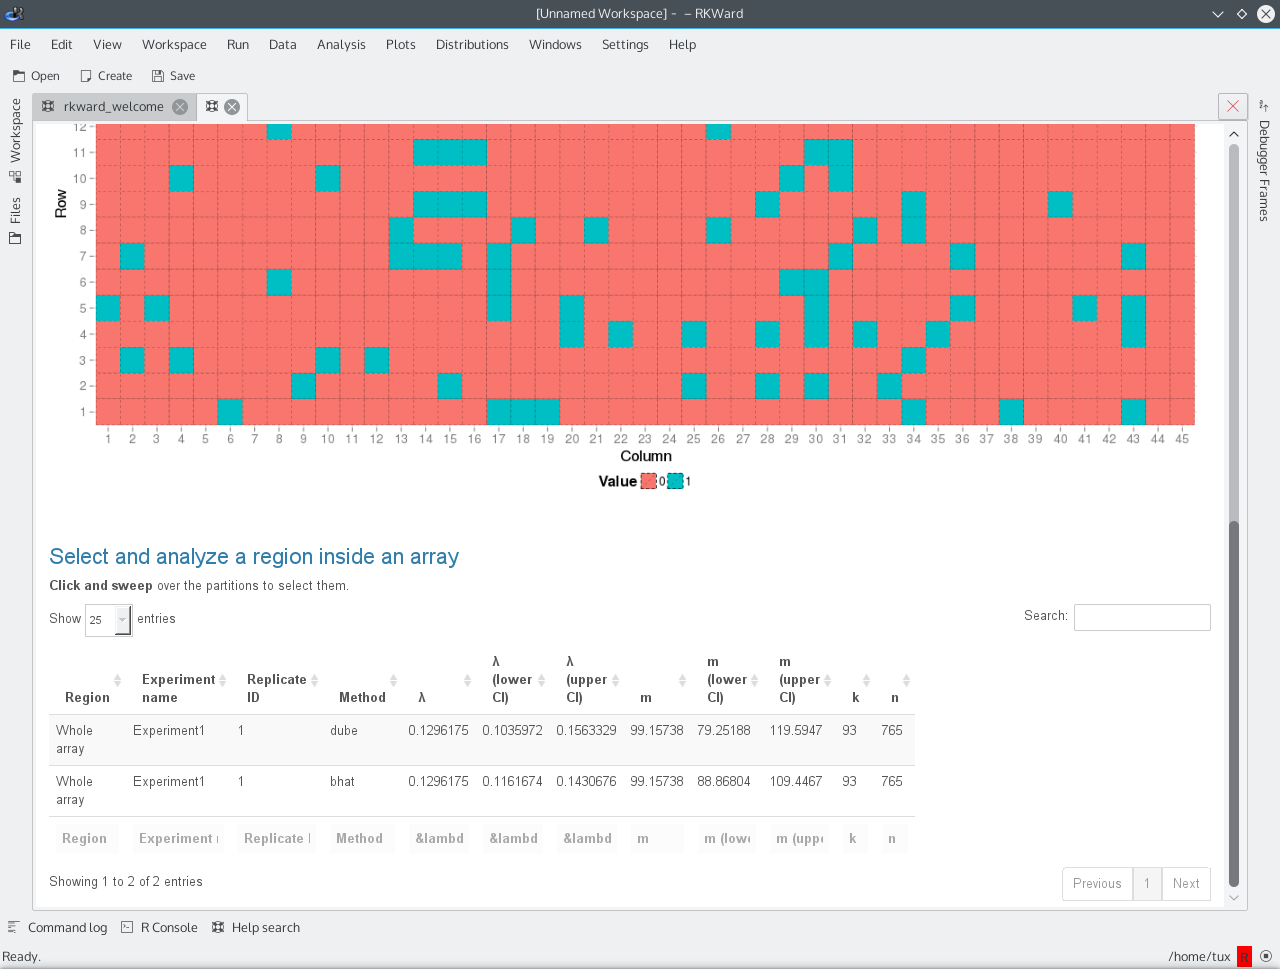
\includegraphics[width=17cm]{GUI_RKWard_1.png}
\end{center}
\caption{\textit{dpcReport()} function running in the graphical user interface 
and integrated development environment \textbf{RKWard}.} 
\label{GUI_RKWard_1}
\end{figure*}




\section{RESULTS}

In the following section we show applications of the \textit{dpcR} package.

\subsection{Vendor independent data analysis}

QX100 series is no longer available. Instead, the newer version QX200 protocol 
consisting of the QX200 droplet generator (Bio-Rad, cat. no. 186-4002) and the 
QX200 droplet reader (Bio-Rad, cat. no. 186-4003) can be purchased, for which 
the protocol can be applied without changes. Alternative dPCR devices available 
from, e.g., RainDance Technologies, Life Technologies or JN Medsys 
\citep{mock_digital_2016}.

\subsection{Automatic report generation}

In \cite{rodiger_r_2015} we gave an example where we re-analyze droplet dPCR 
data from a Bio-Rad QX100 system with an early implementation of the 
\textit{dpcR} package. As recommended in the dMIQE guidelines 
\cite{huggett_digital_2013} we included key elements in the report.

\subsection{Availability}

The \textit{dpcR} framework is available as open source software package (GPL-3 
or later) as part of the Bioconductor project \cite{gentleman_2004}. The stable 
version is hosted at http://cran.r-project.org/web/packages/dpcR and the source 
code is available from  https://github.com/michbur/dpcR.

\section{DISCUSSION}

Currently, there exist different dPCR analysis software solutions provided by 
the vendors. But most of the software packages are black boxes, which prevent 
deep insight into the data processing step. Other and we think that scientific 
software should be open \cite{ince_case_2012, rodiger_r_2015}. In addition, most 
of the software solutions are aimed to be used in very specific scenarios and a 
mutual exclusive to alternative platforms (e.g., droplet vs. chamber-based). We 
have chosen \textbf{R} because it is the \textit{lingua franca} in biostatistics 
and broadly used in other disciplines \cite{rodiger_r_2015}. We developed the 
\textit{dpcR} package, which is a software framework for analysis of dPCR. 
\textit{dpcR} provides the scientific community a broadly applicable tool for 
teaching purposes, data analysis and theoretical research based on simulations. 
Our software framework can be used to accelerate the development of new 
approaches to dPCR.

Functions included may be used to simulate dPCRs, perform statistical data 
analysis, plotting of the results and simple report generation. 

\section{CONCLUSION}

In conclusion, \textit{dpcR} provides means to understand how dPCR works, to 
design, simulate and analyze experiments, and to verify their results (e.g., 
confidence interval estimation), which should ultimately improve 
reproducibility. We have built what we believe to be the first unified, 
cross-platform, dMIQE compliant, open source software framework for analysing 
dPCR experiments. Our \textit{dpcR} framework is targeted at a broad user base 
including end users in clinics, academics, developers, and educators. We 
implemented existing statistical methods for dPCR and suggest the introduction 
of a standardized dPCR nomenclature. Our framework is suitable for teaching and 
includes references for an elaborated set of methods for dPCR statistics. Our 
software can be used for (I) data analysis and visualization in research, (II) 
as software framework for novel technical developments, (III) as platform for 
teaching this new technology and (IV) as reference for statistical methods with 
a standardized nomenclature for dPCR experiments. The framework enables the 
simulations and predictions of Poisson distribution for dPCR scenarios, the 
analysis of previously run dPCRs. Due to the plug-in structure of the software 
it is possible to build custom-made analysers.

Instead of implementing algorithms for clustering and ``rain'' (positive 
droplets) definition of droplet dPCR data, we focused on more specific and not 
yet well-accessible functionalities. We chose not to duplicate existing works 
and instead provide users of dPCR technology with a flexible workflow that 
incorporate most fundamental needs: estimation of the $\lambda$ value, 
comparison of template concentration among several runs and quality control. For 
clustering of ddPCR data, we refer to \textbf{R} packages dedicated to 
flow-cytometer research. Implementations range from manual to automatic 
clustering \cite{le_meur_computational_2013, milbury_determining_2014, 
Malek15022015, trypsteen_ddpcrquant_2015}. 

Moreover, discussion with our peers 
and the literature suggest that a consensus of an appropriate method for dPCR is 
not available \cite{trypsteen_ddpcrquant_2015}.
Our open framework includes to invitation to the scientific community to join 
and support the development of \textit{dpcR}.


\section{ACKNOWLEDGEMENTS}

Grateful thanks belong to the \textbf{R} community and the \textbf{RStudio} 
developers.

\section{Funding}
This work was funded by the InnoProfile-Transfer 03IPT611X (BMBF) and 
KMU-innovativ-16 031B0098B (BMBF) projects.

\subsubsection{Conflict of interest statement.} None declared.
%\newpage

\bibliographystyle{plain}
\bibliography{dpcr}
\end{document}
